\section{Logistic Regression}
    La $\textbf{Logistic Regression}$ è una funzione definita come $$ sig(t) = \frac{1}{1+e^{-t}} $$
    e stima la probabilità che si verifichi un certo evento sulla base di un determinato set di dati di variabili indipendenti.
    
    \begin{figure}[h]
        \caption{Regressione Lineare vs Regressione Logistica}
        \centering
        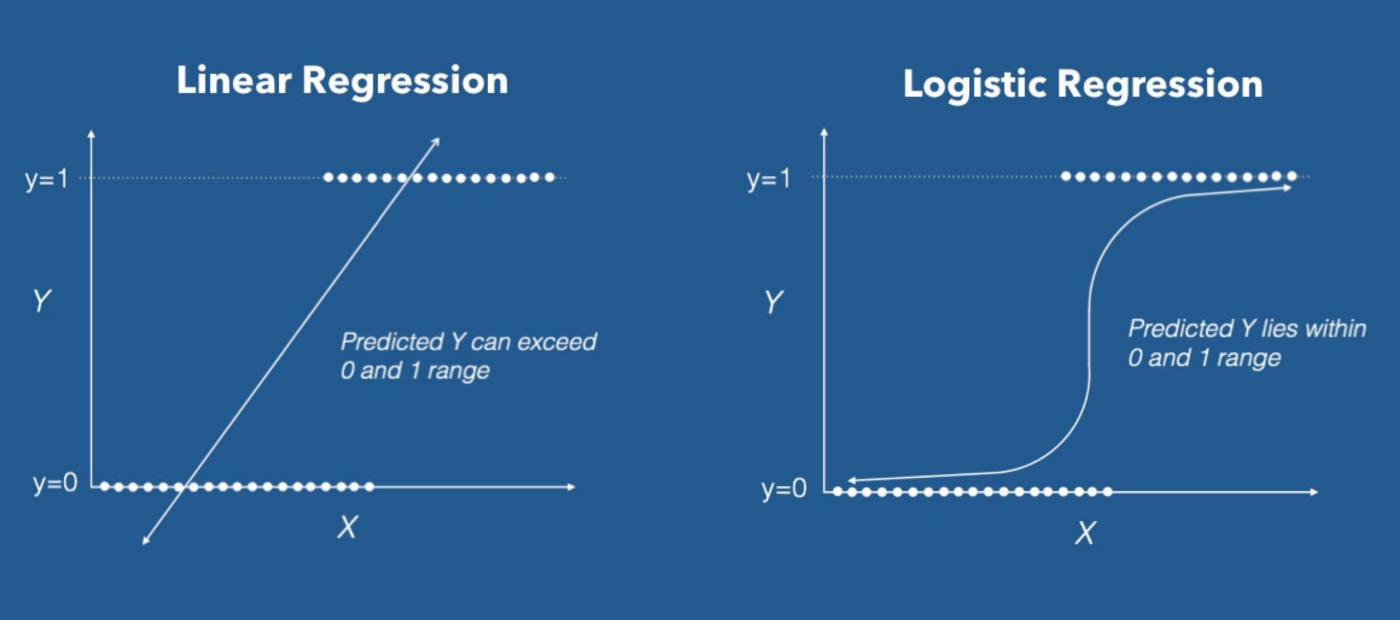
\includegraphics[width = 10cm]{logistic-regression-example.jpeg}
    \end{figure}
    
    \clearpage

    Questo classificatore calcola la retta che separa una classe dall'altra, in uno spazio a due o più dimensioni.
    Tra le infinite rette che possono dividere due classi viene scelta, generalmente, quella che le divide a distanza equa dalla retta.
    È possibile, però, scegliere una retta diversa nel caso si voglia essere più restrittivi verso una classe rispetto a un'altra.
    \\[1\baselineskip]
    $\textbf{NOTA:}$ Poiché il risultato è una probabilità, la variabile dipendente ($Y$) è limitata nell'intervallo $[0,1]$.

    \clearpage